%!TEX root = ../main.tex

\chapter{Photovoltaic Geographical Information System(PGIS)}
\label{chp:Photovoltaic Geographical Information System(PGIS)}

\section{Introduzione al tool(PVGIS)}
Il tool in questione è sviluppato e reso disponibile a titolo gratuito dal \enquote{Joint Research Centre}; Fornice un'interfaccia user friendly per accedere ad un database contenente dati sull'irradianza in differenti locazioni geografiche e permette di calcolare grafici di produzione o di esportare dati specifici sulle condizioni meteo di una determinata zona.\\
E' possibile accedere al \href{https://re.jrc.ec.europa.eu/pvg_tools/it/}{\underline{PVGIS tool}} trovandosi a lavorare con quest'interfaccia:\\
\begin{figure}[H]
    \centering
    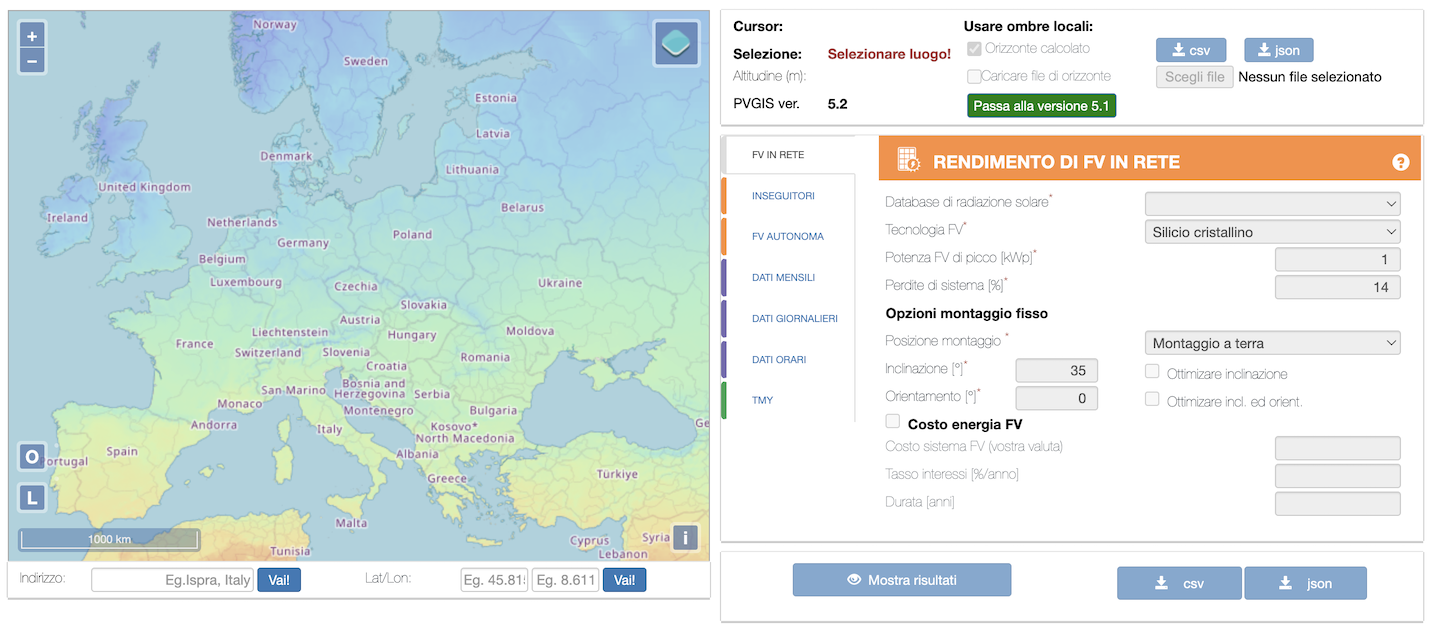
\includegraphics[height=0.5\textwidth]{res/cap 4/PGIS_schermata principale}
    \caption{Interfaccia PVGIS}
\end{figure}\noindent
La prima scelta che va fatta per iniziare ad usar il tool è quella di scegliere una locazione, in questo esempio verrà utilizzata come posizione quella del polo scientifico dell'università di udine(46.081, 13.212).\\
Si procederà poi scegliendo se inserire un file contenente i dati dell'orizzonte o se procedere con un calcolo automatico di esso.
Il primo caso risulta molto comodo quando vi sono ostruzioni naturali od artificiali che possono generare ombra nella superficie che si vuole analizzare.\\
Nel caso si voglia procedere con l'inserimento manuale il programma richiede di inserire una serie di valori, uno per ogni riga, rappresentanti l'altezza dell'orizzonte, misurati in gradi dall'orizzontale.
Le altezze nel file sono considerate ordinante in senso orario partendo da nord, se per esempio si inseriscono quindi 10 valori il programma considera una misurazione ogni $37^\circ$.\\
Una volta operata l'importante scelta riguardo all'orizzonte si può procedere con l'utilizzo del tool.\\
Lo strumento permette di calcolare diverse applicazioni del fotovoltaico e di estrarre diversi parametri meteorologici con cadenza mensile settimanale o giornaliera.
Nel menù laterale possiamo quindi scegliere se di effettuare 3 tipologie di calcoli su ambiti applicativi diversi:
\begin{itemize}
    \item Fotovoltaico in rete
    \item Fotovoltaico ad inseguimento in rete
    \item Fotovoltaico con accumulo
\end{itemize}
Sarà presentata ora una sintetica descrizione delle varie opzioni percorribili
\subsection{Fotovoltaico in rete}
\begin{figure}[H]
    \centering
    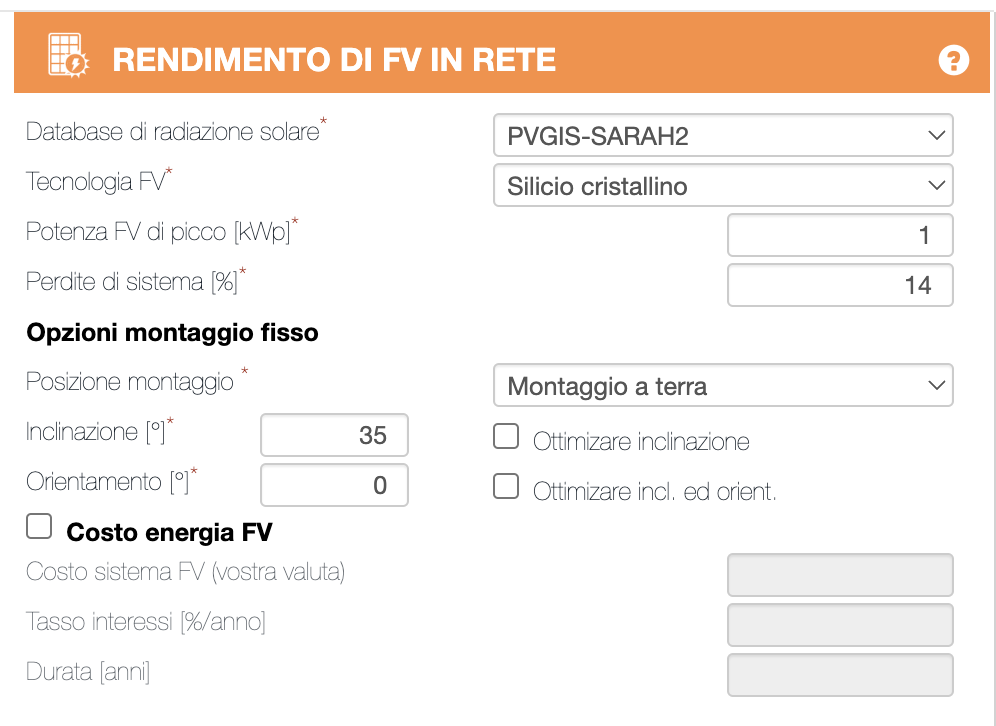
\includegraphics[height=0.5\textwidth]{res/cap 4/Fotovoltaico statico}
    \caption{Scheda fotovoltaico in rete}
\end{figure}\noindent
Come visibile nel'immagine superiore è necessario specificare al sistema diversi parametri quali:
\begin{description}[labelindent=5mm]
    \item[$\bullet$ Database di radiazione solare]: sono proposti tre tipologie di database diversi che si differenziano per range dei dati presenti e per risoluzione che per tutti è inferiore agli \large{$0.5^{\circ}$}
    \item[$\bullet$ Tecnologia fotovoltaico]: sono presenti sia pannelli classici definiti a silicio cristallino che 2 tipologie di moduli a film sottili
    \item[$\bullet$ Potenza di picco]: è la potenza che un modulo è in grado di esprimere ricevendo \large{$1000\frac{W}{m^2}$} perpendicolarmente ad una temperatura di \large{$25^{\circ}C$},è un valore comunque espresso nella scheda tecnica dei moduli fotovoltaici
    \item[$\bullet$ Perdite di sistema]: rappresenta un valore percentuale che esprire tutte le perdire che vanno a ridurre la quantità di energia resa alla rete elettrica, sono incluse in questo valore: perdite resistive dei cavi, perdite dovute all'efficienza dell'inverter, presenza di sporco sui moduli, invecchiamento dei moduli stessi. Il software consiglia automaticamento l'uso di un valore medio di 14\%.
\end{description}
Sono poi da inserire tutte quelle caratteristiche che riguardano l'installazione dell'impianto e sono spesso decise a priori nel caso in cui l'installazione avvenga su un tetto.
\begin{description}[labelindent=5mm]
    \item[$\bullet$ Posizione di montaggio]: i sistema permette di selezionare un montaggio libero, oppure un montaggio su un tetto di un'edificio, nel secondo caso il pannello(a parità di inclinazione) rende meno rispetto al corrispettivo a terra a causa di un minor rendimento dovuto alla temperatura.
    \item[$\bullet$ Inclinazione]: si intende l'angolo che avrà il modulo rispetto all'orizzontale, è possibile lasciare al software il compito di scegliere in autonomia l'inclinazione nel caso non sia un parametro già fissato da fattori fisici
    \item[$\bullet$ Orientamento]: è l'angolo che il modulo avrà rispetto a sud con valori positivi verso ovest e negativi verso est, anche in questo caso l'angolo può essere calcolato in automatico dal software
\end{description}
\vfill
\subsection{Fotovoltaico ad inseguimento in rete}
\begin{figure}[H]
    \centering
    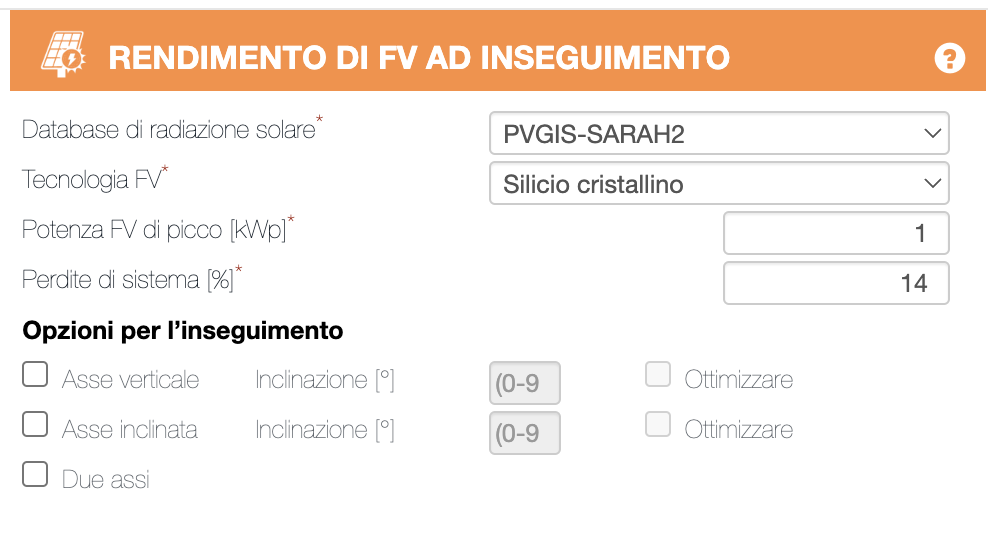
\includegraphics[height=0.5\textwidth]{res/cap 4/moduli ad inseguimento}
    \caption{Scheda fotovoltaico in rete ad inseguimento}
\end{figure}\noindent
Alcuni parametri rimangono identici a quelli illustrati nel caso precedente, a questi si aggiungono:
\begin{description}[labelindent=5mm]
    \item[$\bullet$ Asse verticale]: i moduli sono montati su una struttura con asse di rotazione verticale, l'asse orizzontale è fisso, il suo valore può essere inserito manualmente o calcolato automaticamente.
    \item[$\bullet$ Asse inclinata]: i moduli sono montati su una struttura mobile con un'asse di rotazione inclinata orientata in direzione nord-sud, i moduli vanno montati in modo parallelo all'asse di rotazione, l'inclinazione può essere inserita manualmente o calcolata automaticamente.
    \item[$\bullet$ Due assi]: i moduli sono montati in una struttura mobile su entrambi gli assi quindi risultano totalmente ad inseguimento.
\end{description}
\vfill
\subsection{Fotovoltaico con accumulo}
\begin{figure}[H]
    \centering
    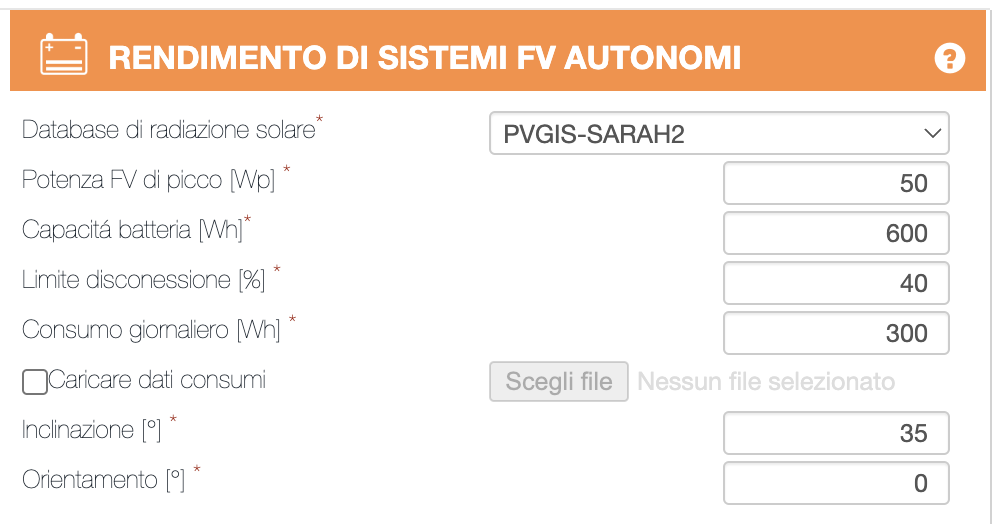
\includegraphics[height=0.5\textwidth]{res/cap 4/fotovoltaico con accumulo}
    \caption{Scheda fotovoltaico con accumulo}
\end{figure}\noindent
In questo caso la scheda risulta diversa dalla precedente in quanto, oltre a tanti parametri trovati nella prima scheda, sono presenti diversi parametri legati alla capacità del stoccaggio disponibile ed al consumo dell'abitazione:
\begin{description}[labelindent=5mm]
    \item[$\bullet$ Capacità batteria]: capacità grezza delle batterie, considerando di poterle scaricare all 100\%
    \item[$\bullet$ Limite di disconnessione]: limite inferire al quale si può scaricare la batteria per evitare di danneggiarla,strettamente legato alla tecnologia della batteria, le batterie al litio ad esempio possono subire una scarica più profonda senza subire danni
    \item[$\bullet$ Consumo giornaliero]: consumo elettrico in un periodo di 24 ore, il software per dividerlo nelle varie ore del giorno utilizza un profilo basato su dati statistici
\end{description}
E' possibile inoltre specificare manualmente il proprio profilo di consumo per rendere i dati più veritieri per il proprio uso
\subsection{Export dati mensile}
\begin{figure}[H]
    \centering
    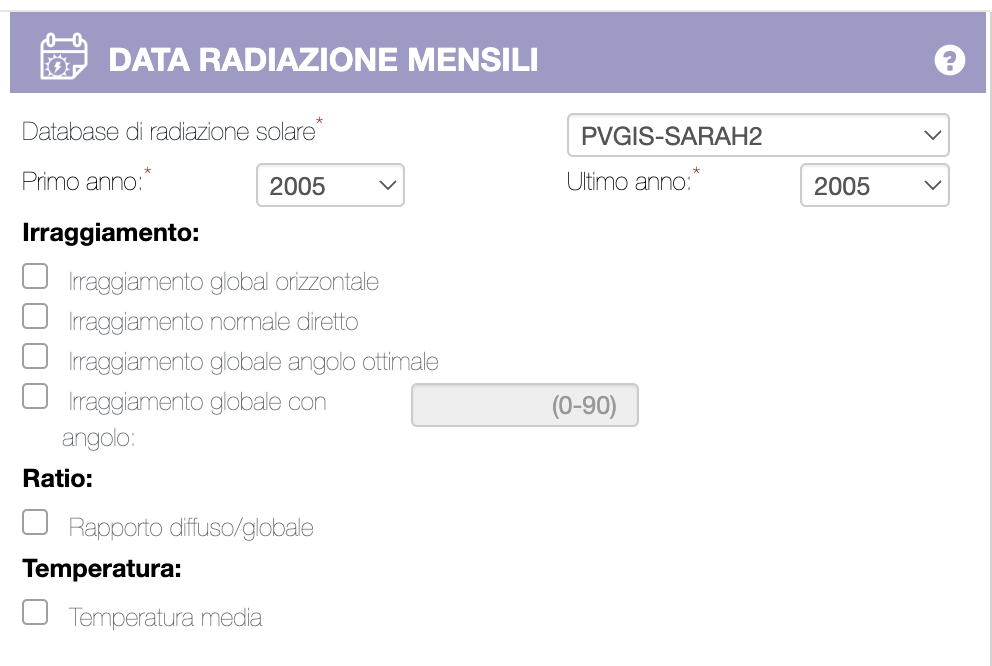
\includegraphics[height=0.5\textwidth]{res/cap 4/dati mensili}
    \caption{Scheda dati mensili}
    \label{fig:export mensile}
\end{figure}\noindent
Tramite questa scheda una volta selezionato l'orizzonte temporaneo da prendere in analisi, il range disponibile dipende dal modello scelto, per quello presente in'immagine ad esempio sono presenti dati dal 2005 al 2020.
L'export può comprendere tutti i dati in figura:
\begin{description}[labelindent=5mm]
    \item[$\bullet$ Irraggiamento globale orizzontale]: rappresenta la somma mensile dell'energia delle radiazioni su ogni metro quadro di piano orizzontale
    \item[$\bullet$ Irraggiamento normale diretto]: rappresenta la somma mensile dell'energia delle radiazione su un piano che segue il sole in modo da puntarlo sempre direttamente, include le sole radiazioni provenienti direttamente dal sole e non quelle che arrivano per altri fenomeni.
    \item[$\bullet$ Irraggiamento globale con angolo ottimale]: rappresenta la somma mensile dell'energia delle radiazioni su ogni metro quadro di un piano rivolto verso l'equatore ed inclinato così che riceve il massimo dell'energia durante l'anno.
    \item[$\bullet$ Irraggiamento globale con angolo scelto dall'utente]: come nel caso precendete solo che l'angolo invce di esssere sempre ottimale è definito dall'utente
    \item[$\bullet$ Rapporto tra radiazione diffusa e globale]: rappresenta la media mensile del rapporto tra la radiazione diffusa e quella globale, un valore alto è tendenzialmente indice di un clima nuvoloso.
\end{description}
\subsection{Export dati giornalieri}
\begin{figure}[H]
    \centering
    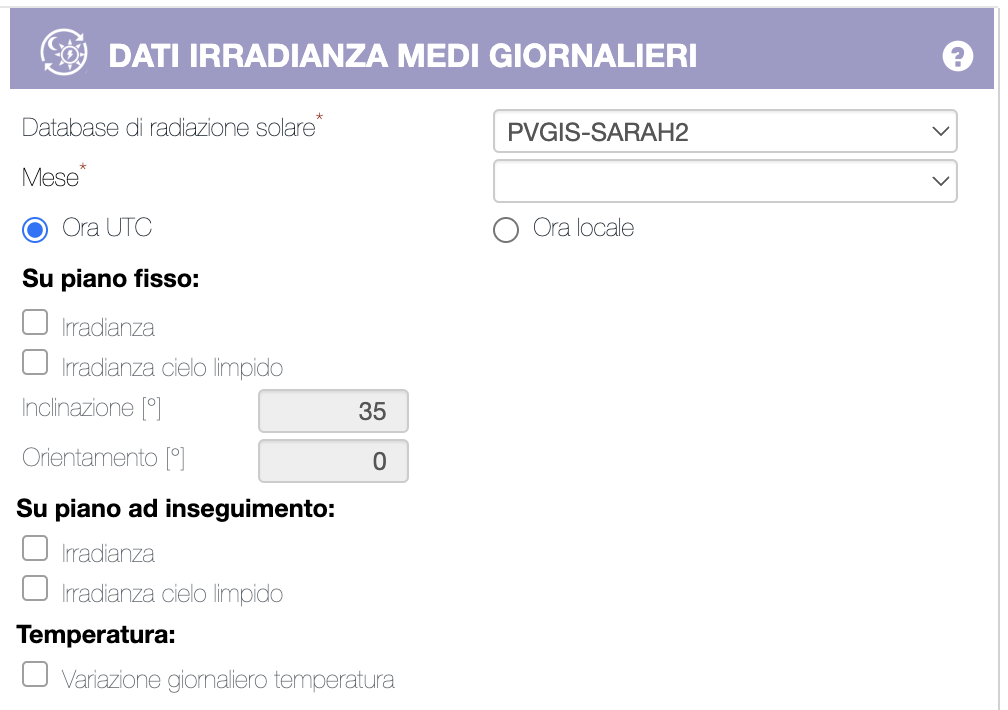
\includegraphics[height=0.5\textwidth]{res/cap 4/dati giornalieri}
    \caption{Scheda dati giornalieri}
\end{figure}\noindent
Tramite questa scheda una volta selezionato il mese che si intende valutare  ed il modello da utilizzare.
Questa scheda risulta molto comoda per confrontare soluzioni fisse con soluzioni ad inseguimento, per entrambe si possono ottenere dati sull'irradianza con cielo sia considerando che non la nuvolosità del cielo

\subsection{Export dati orario}
\label{subsec:export orario}
\begin{figure}[H]
    \centering
    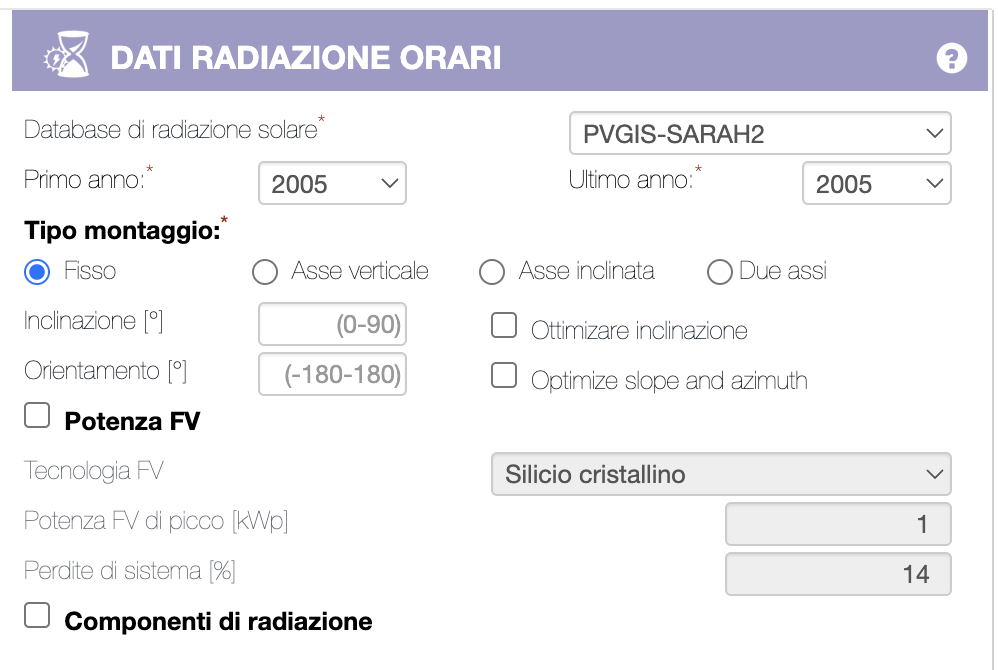
\includegraphics[height=0.5\textwidth]{res/cap 4/dati orari}
    \caption{Scheda dati orari}
\end{figure}\noindent
Tramite questa scheda una volta selezionato l'orizzonte temporaneo da prendere in analisi, il range disponibile dipende dal modello scelto, per quello presente in'immagine ad esempio sono presenti dati dal 2005 al 2020.
Prima di effettuare l'export bisogna selezionare il tipo di montaggio che si intende analizzare ed i parametri costruttivi.
Si ottiene in output un file contenente i vari timeframe, la potenza,l'irradianza nel piano scelto, l'altezza del sole,la temperatura dell'aria ed il vento a 10 metri dal suolo.
Spuntando anche l'output delle singole componenti si ottengono dati più dettagliati sulle componenti: diffusa, diretta e riflessa.

\subsection{Esempio di export di dati}
Sarà ora presentato un'esempio dei dati ottenibili per un'impianto fotovoltaico posizionato a terra in un terreno adiacente all'università.
Tutte le simulazione hanno in comune un grafico riportante l'orizzonte nelle diverse direzioni e l'angamento del sole, esso è molto utile per, ad esempio, poter effettuare una scelta più ponderata sull'orientazione dei moduli fotovoltaici.
\begin{figure}[H]
    \centering
    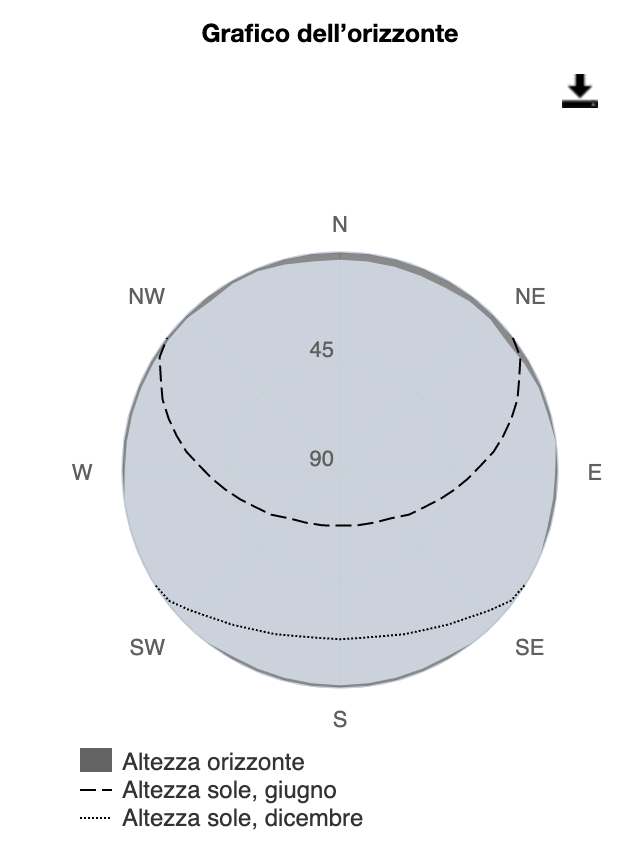
\includegraphics[height=0.5\textwidth]{res/cap 4/orizzonte}
    \caption{Diagramma contenente linea orizzonte ed altezza sole}
    \label{fig:orizzonte}
\end{figure}\noindent
Dal diagramma possiamo notare come la posizione scelta non subisca interferenza di ostruzioni naturali(montagne, colline), se si volesse tracciare anche l'interferenza di elementi più piccoli bisognerebbe inserire manualmente un profilo dell'orizzonte.
La simulazione sarà effettuata con per un'impianto tradizionale da 1Kwp inizialmente lasciando definire gli angoli di inclinazione e orientamento al software.
\begin{figure}[H]
    \centering
    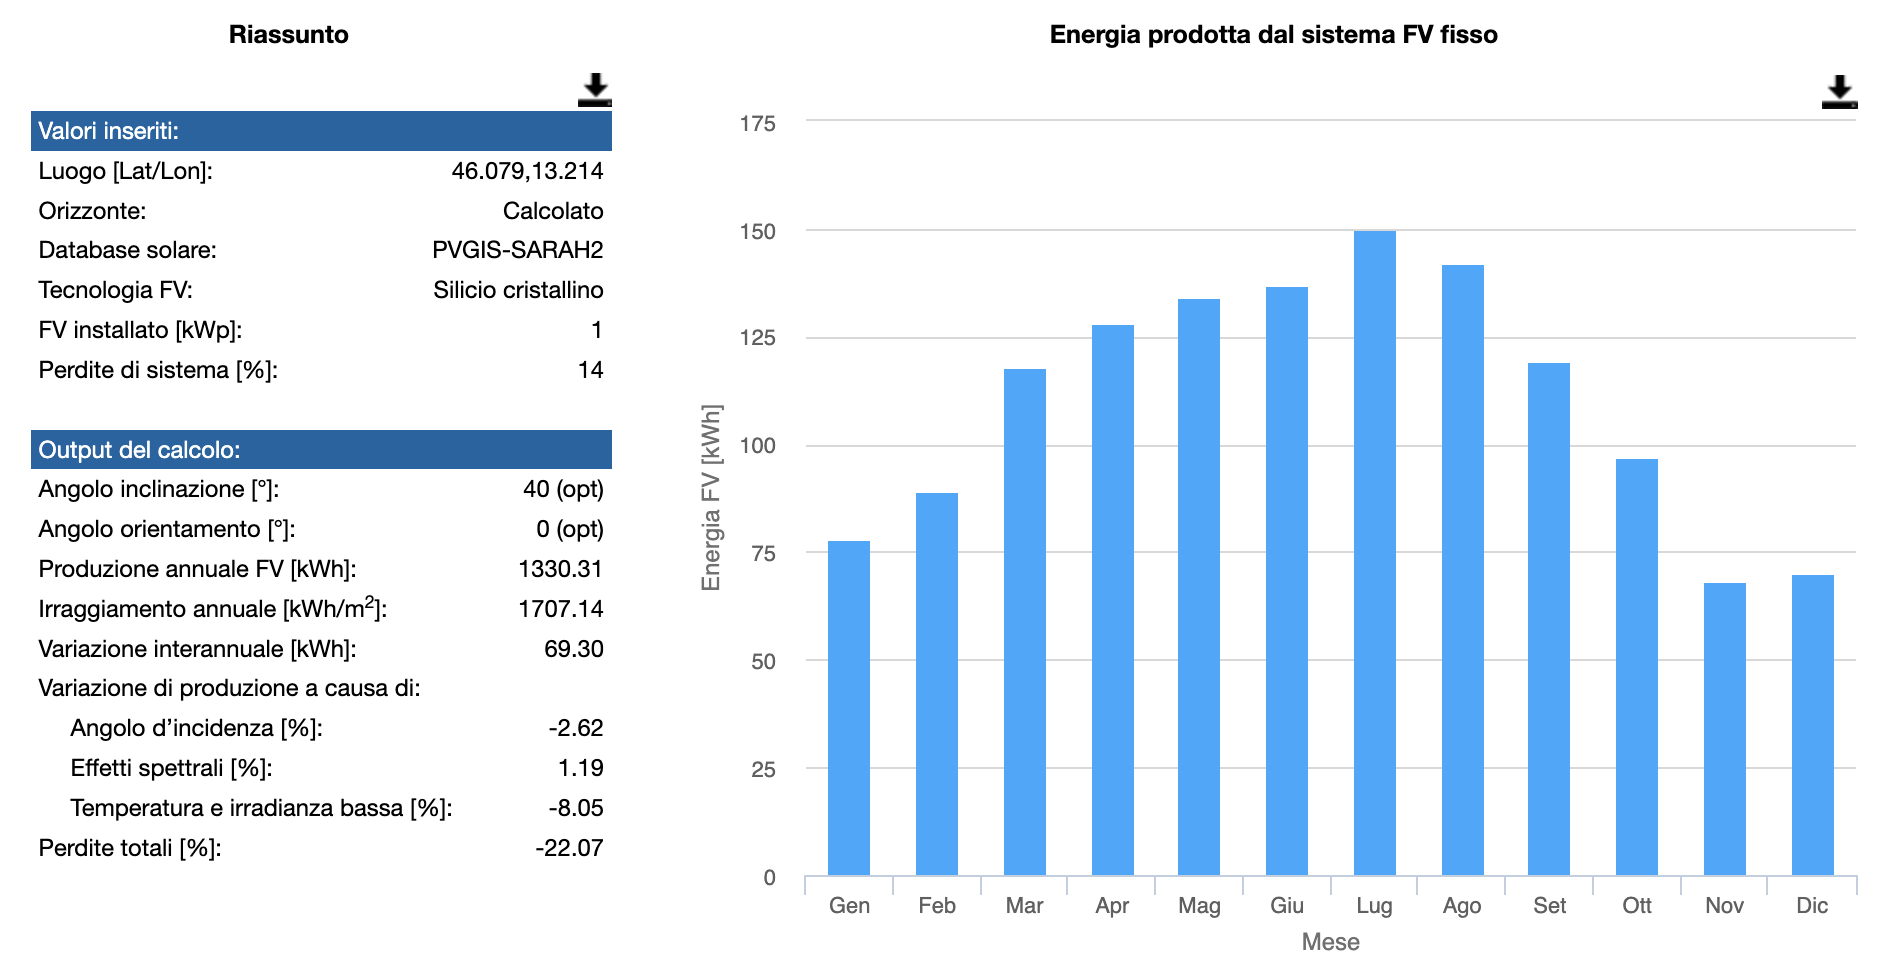
\includegraphics[height=0.5\textwidth]{res/cap 4/fissi uniud-auto}
    \caption{Export dati modulo fisso con orientazione automatica}
    \label{fig:export}
\end{figure}\noindent
Si può notare come il software abbia ovviamente orientato i moduli a sud, l'angolo è stato scelto per avere una resa media ottima in tutto l'anno.
Scegliere un'angolo minore incrementerebbe la produzione nei mesi estivi ma porterebbe un netto peggioramento in quelli invernali, un'inclinazione superiore ai 40 gradi invece gioverebbe nel periodo invernale ma sarebbe peggiorativa in quello estivo.
Procediamo ora con l'analisi di un'impianto ad inseguimento, lasciamo anche in questo caso al software la definizione degli angoli e in modo da poter confrontare nel caso ottimo le tre tipologie di impianti ad inseguimento.
\begin{figure}[H]
    \centering
    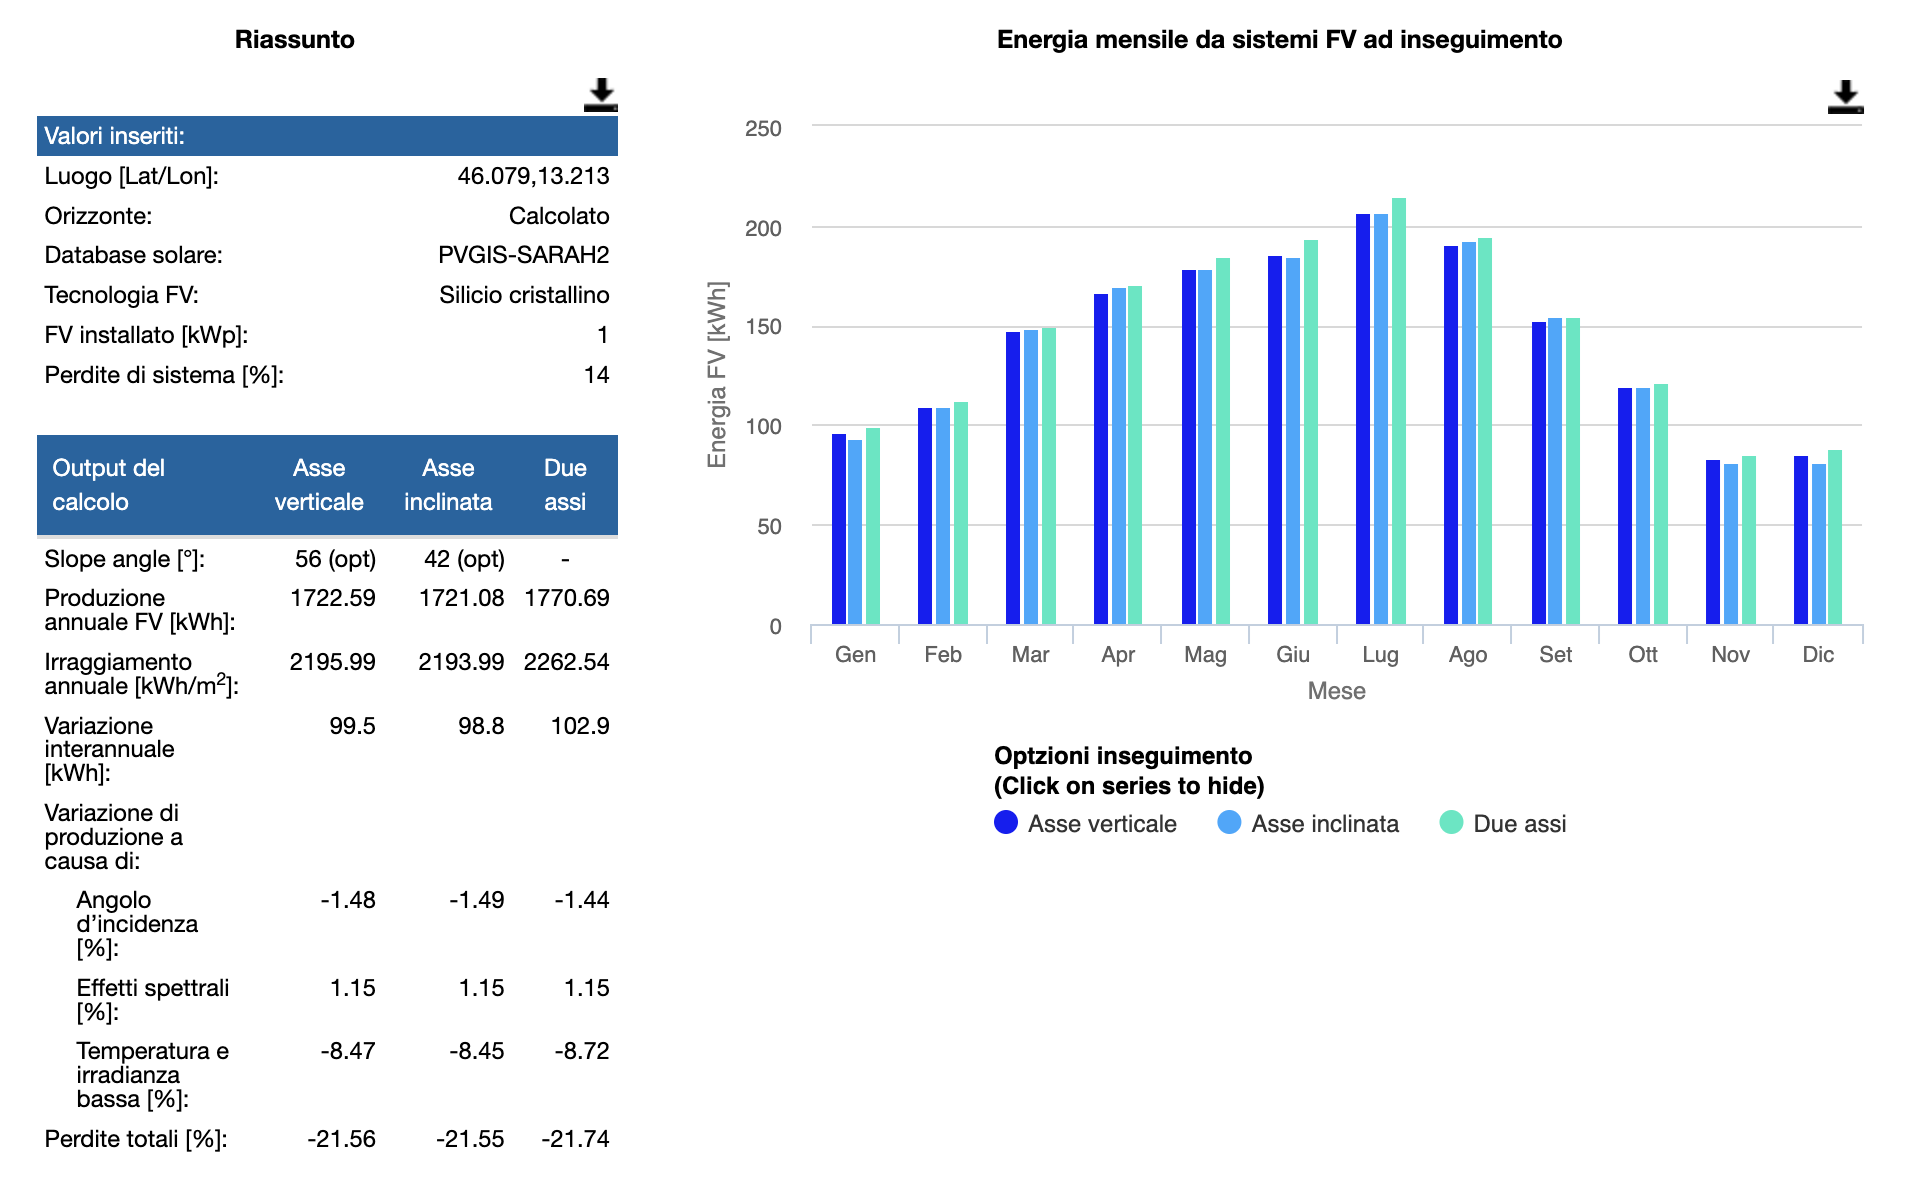
\includegraphics[height=0.6\textwidth]{res/cap 4/inseguimento uniud-auto}
    \caption{Export dati modulo fisso con orientazione automatica}
\end{figure}\noindent
Si nota come la produzione sia nettamente superiore al caso di moduli fissi e potendo orientare tutti gli assi ci sia un'ulteriore guadagno.
Il caso di impianto con accumulo non sarà trattato in quanto non di interesse per questa tesi.
